\documentclass{article}\usepackage[]{graphicx}\usepackage[]{color}
%% maxwidth is the original width if it is less than linewidth
%% otherwise use linewidth (to make sure the graphics do not exceed the margin)
\makeatletter
\def\maxwidth{ %
  \ifdim\Gin@nat@width>\linewidth
    \linewidth
  \else
    \Gin@nat@width
  \fi
}
\makeatother

\definecolor{fgcolor}{rgb}{0.345, 0.345, 0.345}
\newcommand{\hlnum}[1]{\textcolor[rgb]{0.686,0.059,0.569}{#1}}%
\newcommand{\hlstr}[1]{\textcolor[rgb]{0.192,0.494,0.8}{#1}}%
\newcommand{\hlcom}[1]{\textcolor[rgb]{0.678,0.584,0.686}{\textit{#1}}}%
\newcommand{\hlopt}[1]{\textcolor[rgb]{0,0,0}{#1}}%
\newcommand{\hlstd}[1]{\textcolor[rgb]{0.345,0.345,0.345}{#1}}%
\newcommand{\hlkwa}[1]{\textcolor[rgb]{0.161,0.373,0.58}{\textbf{#1}}}%
\newcommand{\hlkwb}[1]{\textcolor[rgb]{0.69,0.353,0.396}{#1}}%
\newcommand{\hlkwc}[1]{\textcolor[rgb]{0.333,0.667,0.333}{#1}}%
\newcommand{\hlkwd}[1]{\textcolor[rgb]{0.737,0.353,0.396}{\textbf{#1}}}%

\usepackage{framed}
\makeatletter
\newenvironment{kframe}{%
 \def\at@end@of@kframe{}%
 \ifinner\ifhmode%
  \def\at@end@of@kframe{\end{minipage}}%
  \begin{minipage}{\columnwidth}%
 \fi\fi%
 \def\FrameCommand##1{\hskip\@totalleftmargin \hskip-\fboxsep
 \colorbox{shadecolor}{##1}\hskip-\fboxsep
     % There is no \\@totalrightmargin, so:
     \hskip-\linewidth \hskip-\@totalleftmargin \hskip\columnwidth}%
 \MakeFramed {\advance\hsize-\width
   \@totalleftmargin\z@ \linewidth\hsize
   \@setminipage}}%
 {\par\unskip\endMakeFramed%
 \at@end@of@kframe}
\makeatother

\definecolor{shadecolor}{rgb}{.97, .97, .97}
\definecolor{messagecolor}{rgb}{0, 0, 0}
\definecolor{warningcolor}{rgb}{1, 0, 1}
\definecolor{errorcolor}{rgb}{1, 0, 0}
\newenvironment{knitrout}{}{} % an empty environment to be redefined in TeX

\usepackage{alltt}
\usepackage{cite}

\usepackage{amsmath}
\usepackage{amsthm}
\usepackage{graphicx, epsfig}
\usepackage{amssymb}
\usepackage{natbib}
\usepackage[ruled, vlined]{algorithm2e}

\newtheorem{theorem}{Theorem}
\newtheorem{lemma}{Lemma}
\DeclareMathOperator{\tr}{tr}
\DeclareMathOperator{\diag}{diag}
\DeclareMathOperator{\sign}{sign}
\DeclareMathOperator{\ifelse}{ifelse}
\DeclareMathOperator{\Unif}{Unif}
\DeclareMathOperator{\snr}{snr}
\newtheorem{corollary}{Corollary}
\newtheorem{proposition}{Proposition}

\IfFileExists{upquote.sty}{\usepackage{upquote}}{}
\begin{document}
\section{A Mixture of Mixed GLMs}
\subsection{Mixed Binomial Regression}
Cell count data exhibits over-dispersion when compared to what would be expected from a standard binomial experiment. This can be seen in Figure \ref{CD154scatter} where the diagonal line serves as a baseline proportion for each subject. Subjects in the control group tend to be close to the diagonal line and subjects in the treatment group tend to be above the diagonal line (because the stimulated sample has a higher count of cells than the unstimulated sample).

\begin{figure}
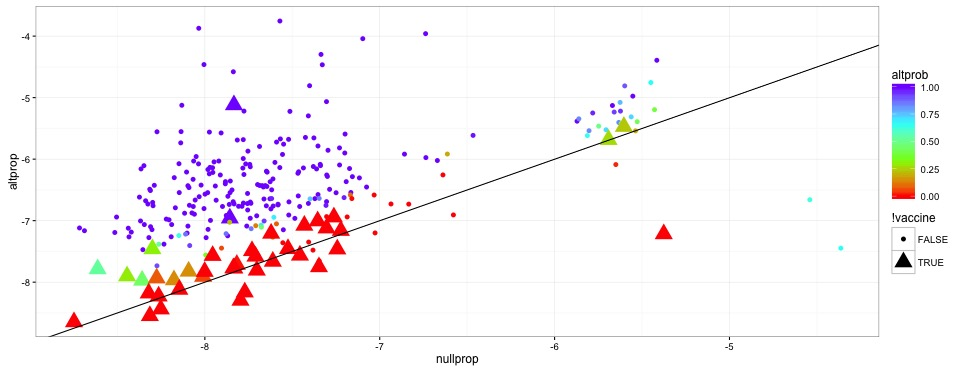
\includegraphics[width=\maxwidth]{figures/T4CD154scatter} \caption[]{Scatter plot of the log-proportions for the T4+/CD154 cell-subset. The x-axis is the log proportion in the control sample and the y-axis is the log proportion in the stimulated sample. Subject in the control group are marked with triangles and subject in treatment group as circles. The posterior probability of being a responder (or in the treatment group) is marked by color, purple being a probability close to one and red a posterior probability close to zero.}
\label{CD154scatter}
\end{figure}

While the Beta-Binomial distribution is a good model for over-dispersion when the over-dispersion is observed at the blood-sample level, here most of the over-dispersion seems to be at the subject-level and when this variability is accounted for the over-dispersion observed at the sample level is actually very small. We can model the count of a specific blood cell type in the $j$th sample from the $i$th subject with the following model:
$$
y_{ij} \sim \text{Bin}(N_{ij}, p_{ij}),
$$$$
\text{logit}(p_{ij}) = X_{ij} \beta + \nu_{i},
$$$$
\nu_{i} \sim N(0, \sigma^{2}).
$$
Giving rise to the likelihood:
$$
f(y_{i}) = \int_{\mathbb{R}} \prod_{j} f(y_{ij} ; X_{ij}, \beta, \nu) \varphi(\nu;\sigma^{2})d\nu.
$$
There are many existing software packages for fitting such regression models which work well as long as the dimension of the integral is not too big ($\leq 3$).

\subsection{A Finite Mixture Of Mixed Regression}
In addition to accounting for over-dispersion we must also account for the fact that we may have non-responders in our study. To account for that we can use the following model:
$$
y_{ij} \sim \pi_0\text{Bin}(N_{ij}, p_{ij0}) + \pi_1\text{Bin}(N_{ij}, p_{ij1}),
$$$$
\pi_0 + \pi_1 = 1,
$$$$
\text{logit}(p_{ijk}) = X_{ij} \beta + T_{ij}\tau_{k} + \nu_{i},
$$$$
\nu_{i} \sim N(0, \sigma^{2}),
$$$$
\tau_{k} = \begin{cases}
\tau & k = 1 \\
0 & k = 0 
\end{cases}.
$$
Where $X_{ij}$ and $T_{ij}$ are known matrices, $\tau_k$ is a random regression coefficient that equals either zero or an unknown constant (which needs to be estimated).

We can estimate this model using an SEM algorithm (Stochastic-EM). In the E-step we approximate the posterior probability of belonging to the $k$th cluster based on the observed data and current set of parameters:
$$
\pi_{i0} = \frac{f_0(y_{i}) \pi_0}{f_0(y_{i})\pi_0 + f_1(y_{i})\pi_1},
$$$$
\pi_{i1} = 1 - \pi_{i0},
$$$$
f_k(y_{i}) = \int_{\mathbb{R}} \prod_{j} f(y_{ij} ; X_{ij}, T_{ij}, \tau_k, \beta, \nu) \varphi(\nu;\sigma^{2})d\nu.
$$
In the M-step, we maximize the complete data log-likelihood:
$$
\sum_{k=0}^{1}\sum_{i=1}^{n} \pi_{ik}\log f_k(y_i) + \pi_{ik} \log \pi_{k},
$$
given the posterior probabilities $p_{ik}$ this can be done using a standard mixed modeling library (such as \textbf{lme4}). 

The reason we need to use a Stochastic-EM algorithm rather than a standard EM is that in the in the E-step the posterior probabilities are not given in closed form and they must be approximated. We approximate them using a importance sampling scheme. For the $i$th subject and for $k\in \{0, 1\}$ we sample $v_{k1},...v_{kM} \sim N(\mu_{ik}, \sigma^{2})$, where $\mu_{ik}$ is estimated as a part of the M-step. We then compute an approximation to the posterior probability:
$$
\frac{f_0(y_{i}) \pi_0}{f_0(y_{i})\pi_0 + f_1(y_{i})\pi_1} 
= \left(1 + \frac{\pi_1}{\pi_0}\frac{f_1(y_{i})}{f_0(y_i)} \right)^{-1}
$$$$
\approx  \left(1 + \frac{\pi_1}{\pi_0}
\frac{\sum_{m=1}^{M} \frac{\varphi(v_{1m};0,\sigma^{2})}{\varphi(v_{1m}; \mu_{i1}, \sigma^{2})}\prod_{j} f_1(y_{ij} ; v_{m})}
{\sum_{m=1}^{M}\frac{\varphi(v_{0m};0,\sigma^{2})}{\varphi(v_{0m}; \mu_{i0}, \sigma^{2})} \prod_{j} f_0(y_{ij} ; v_{m})} 
\right)^{-1} 
:= w_{i0}.
$$
Since $w_{ik}$ is only a rough approximation for $p_{ik}$,  we update the posterior probabilities gradually:
$$
\pi_{ik}^{t} = \pi_{ik}^{t-1} + \frac{(w_{ik} - \pi_{ik}^{t-1})}{\sqrt{t}}.
$$

\section{Some Data Analysis}
\subsection{Modeling with a Single Random Effect}
Let us fit this model to the RV144 dataset. Figure \ref{CD154scatter} describe the distribution of the log-proportions of T4+/CD154 cells in the two stimulus types and the posterior probabilities of being responders assigned by the algorithm to the subjects. The model assigns high probabilities to observations above the $x=y$ line and low probabilities to observations close to the line or below it. In Figure \ref{CD154roc} we plot the ROC curve and nominal-FDR vs. empirical-FDR for the T4+/CD154 cell subset. The AUC is $0.921$ and the False-Detection rate is controlled while maintaining good power. 

\begin{figure}
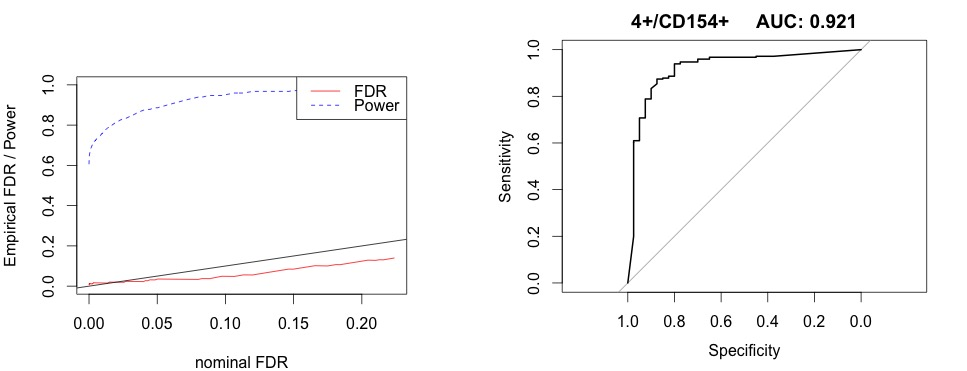
\includegraphics[width=\maxwidth]{figures/T4CD154roc} \caption[]{ROC and False Detection Rate for the T4+/CD154 cell subset.}
\label{CD154roc}
\end{figure}

In Figure \ref{IFNG} we plot the scatterplot, ROC and FDR for the T4+/IFNG+ cell-subset. Here the FDR is still good but the AUC is a lower of $0.87$. This can be improved if we fit a model to the IFNG+ and  CD154 cell-subsets together. At the moment, it is only possible to fit models with a single subject-level random effect.  However, this works well enough in this case because, as we will show, the random effects in these two cell-subsets are highly correlated. The classification error and posterior probabilities given by the joint model are presented in Figure \ref{jointModel}.

\begin{figure}
\includegraphics[width=\maxwidth]{figures/t4ifngroc} 
\includegraphics[width=\maxwidth]{figures/t4ifngscatter} \caption[]{Plots for the T4+/IFNG+ cell subset.}
\label{IFNG}
\end{figure}

\begin{figure}
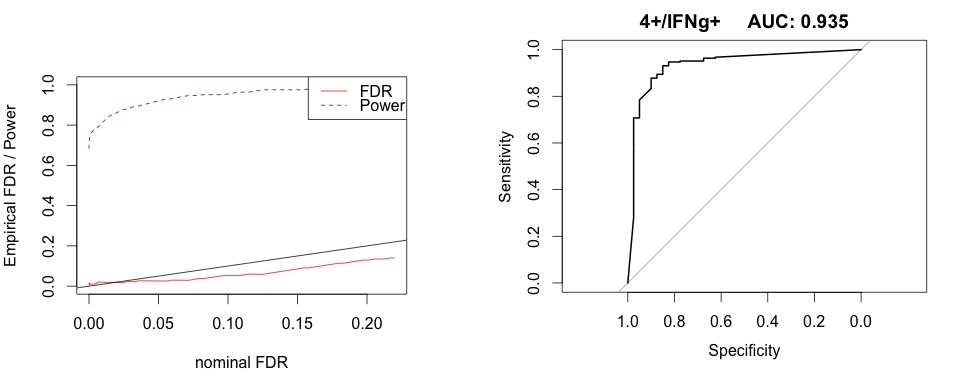
\includegraphics[width=\maxwidth]{figures/jointroc} 
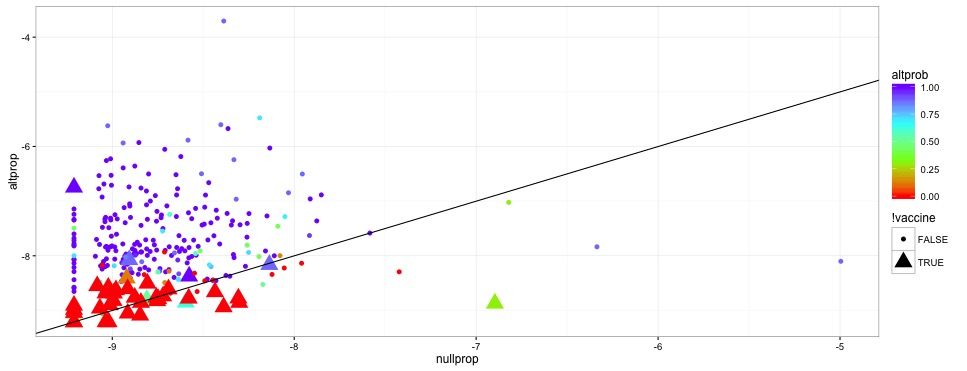
\includegraphics[width=\maxwidth]{figures/jointscatter} \caption[]{Posterior probabilities and classification errors for the joint model of T4+/CD154 and T4+/IFNG+. The scatter plot is for log proportions of the T4+/IFNG+ cell-subset.}
\label{jointModel}
\end{figure}

Joint modeling for multiple cell-subsets may fail if some of the random effects have different distributions. As we show in Figure \ref{IL4}, this is the case if we try to model the T4+/CD154 and T4+/IL4+ cell-subsets with one random effect. Here, the classification is worse than the one classification we would get had we fit a model for the T4+/CD154 cell subset alone.

\begin{figure}
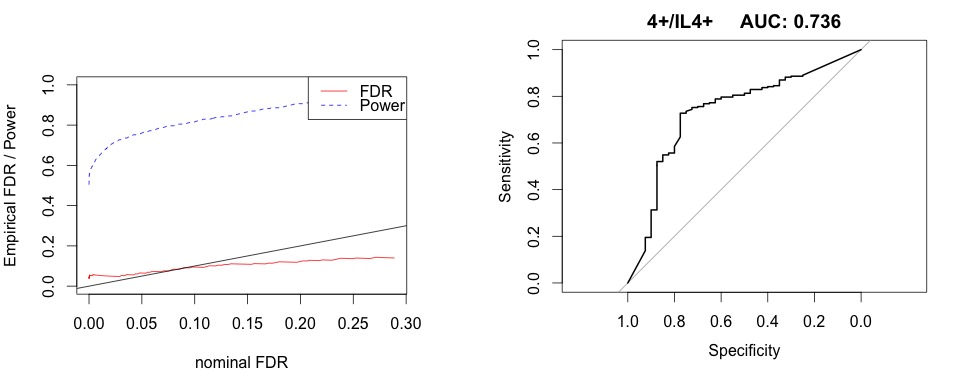
\includegraphics[width=\maxwidth]{figures/IL4jointRoc} 
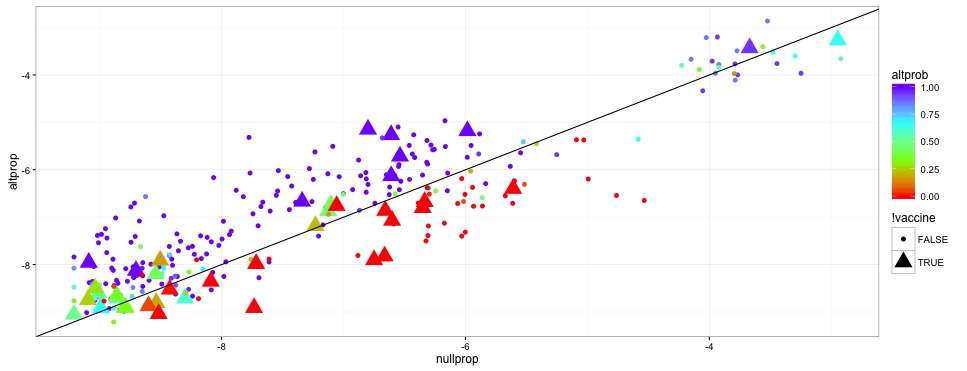
\includegraphics[width=\maxwidth]{figures/IL4jointScatter} \caption[]{Posterior probabilities and classification errors  for the joint model of T4+/CD154 and T4+/IL4+. The scatter plot is for log proportions of the T4+/IL4+ cell-subset.}
\label{IL4}
\end{figure}






\subsection{Dependence Between Cell-Subsets}
From the single random-effect analysis we learn that:
\begin{itemize}
\item It is beneficial to model multiple cell-subsets at the same time. Joint modeling can improve the subject analysis as well as (probably) the global effect estimates.
\item Univariate random-effects are only suitable to modeling highly correlated cell subsets. 
\end{itemize}

In order to better understand the dependence structure we can expect to see in this sort of datasets, we fit the following model to all pairs of T4+ cell types in the RV144 dataset. For the $l$th cell-subset, $j$th sample from the $i$th subject: 
$$
\text{logit}(p_{ijl}) = \beta_{0l} + 
\text{stim}_{j} * \beta_{1l} + \text{vaccine}_{i}*\beta_{2l} 
+ \text{stim}_j * \text{vaccine}_i * \beta_{3l} + \nu_{il},
$$$$
\nu_{i} \sim N_2(0, \Sigma).
$$
The fitting procedure (as implemented in \textbf{lme4}) return the estimated covariance structure in each pairwise model. The resulting covariance and correlation structures are given in Tables \ref{covTable} and \ref{corTable} respectively. The highest correlations in the tables are between the four cell-subsets where there is a strong visible vaccine effect- CD154+, IFNg+, IL2+ and TNFa+. However, there are is some degree of non-negligible correlation between most cell-subsets. 

\begin{table}[ht]
\centering
\begin{tabular}{rrrrrrrr}
  \hline
 & 1 & 2 & 3 & 4 & 5 & 6 & 7 \\ 
  \hline
4+/CD154+ & 0.63 & 0.53 & 0.39 & 0.55 & 0.44 & 0.38 & 0.47 \\ 
  4+/IFNg+ & 0.53 & 0.69 & 0.44 & 0.31 & 0.29 & 0.20 & 0.53 \\ 
  4+/IL2+ & 0.39 & 0.44 & 0.39 & 0.13 & 0.23 & 0.11 & 0.47 \\ 
  4+/IL4+ & 0.55 & 0.31 & 0.13 & 3.13 & 0.95 & 0.61 & 0.18 \\ 
  4+/IL17a+ & 0.44 & 0.29 & 0.23 & 0.95 & 0.75 & 0.38 & 0.36 \\ 
  4+/MIP1B+ & 0.38 & 0.20 & 0.11 & 0.61 & 0.38 & 1.47 & 0.21 \\ 
  4+/TNFa+ & 0.47 & 0.53 & 0.47 & 0.18 & 0.36 & 0.21 & 0.68 \\ 
   \hline
\end{tabular}
\caption{Covariance Between Random Effects in the RV144 Dataset.}
\label{covTable}
\end{table}

\begin{table}[ht]
\centering
\begin{tabular}{rrrrrrrr}
  \hline
 & 1 & 2 & 3 & 4 & 5 & 6 & 7 \\ 
  \hline
4+/CD154+ & 1.00 & 0.80 & 0.78 & 0.39 & 0.64 & 0.40 & 0.72 \\ 
  4+/IFNg+ & 0.80 & 1.00 & 0.85 & 0.21 & 0.40 & 0.20 & 0.77 \\ 
  4+/IL2+ & 0.78 & 0.85 & 1.00 & 0.12 & 0.42 & 0.15 & 0.92 \\ 
  4+/IL4+ & 0.39 & 0.21 & 0.12 & 1.00 & 0.62 & 0.29 & 0.13 \\ 
  4+/IL17a+ & 0.64 & 0.40 & 0.42 & 0.62 & 1.00 & 0.37 & 0.51 \\ 
  4+/MIP1B+ & 0.40 & 0.20 & 0.15 & 0.29 & 0.37 & 1.00 & 0.21 \\ 
  4+/TNFa+ & 0.72 & 0.77 & 0.92 & 0.13 & 0.51 & 0.21 & 1.00 \\ 
   \hline
\end{tabular}
\caption{Correlations Between Random Effects in the RV144 Dataset.}
\label{corTable}
\end{table}





\section{Modeling with a Multivariate Random-Effect Distribution}
Let $y_{ijl}$ denote the count for the $l$th cell subset in the $j$th stimulation from the $i$th subject. We wish to estimate the model:
$$
y_{ijl} \sim \pi_0 Bin(N_{ij}, p_{ijl0}) + \pi_1 Bin(N_{ij}, p_{ijl1})
$$$$
\pi_0 + \pi_1 = 1,
$$$$
\text{logit}(p_{ijlk}) = X_{ijl} \beta_l + T_{ijl}\tau_{lk} + \nu_{il},
$$$$
\nu_{i} \sim N_L(0, \Sigma),
$$$$
\tau_{kl} = \begin{cases}
\tau_l & k = 1 \\
0 & k = 0 
\end{cases}.
$$
Where $X_{ijl}$ and $T_{ijl}$ are known matrices, $\tau_{lk}$ is a random regression coefficient that equals either zero or an unknown constant (which needs to be estimated). The likelihood of the model is given by:
$$
\mathcal{L}(\beta,\tau, \pi, \Sigma; y) = \prod_{i=1}^{n}\left[
\sum_{k=0}^{1} \pi_k\int_{\mathbb{R}^{L}} \prod_{jl} f(y_{jl} |\tau_k, \beta, \nu_i) \varphi(\nu_i;\Sigma) d\nu_i
\right].
$$

\subsection{Estimating the Mixed-Multivariate-Mixed-Effect-Model}
The likelihood is non-trivial to maximize because it includes both a summation and a high-dimensional integral. In order to do so, we will use a nested Monte-Carlo EM algorithm where we have an outer MCEM algorithm, the M-step of which is itself an MCEM. Write the full-information log-likelihood for the mixture model:
$$
l(\beta, \tau, \Sigma | \pi_{1,...,n}) = \sum_{i=1}^{n} \sum_{k=0}^{1}\pi_{ik} \log \int_{\mathbb{R}^{L}} \prod_{jl} f(y_{jl} |\beta, \tau_k, \nu_i) \varphi(\nu_i;\Sigma)d\nu_i + \pi_{ik}\log \pi_k
$$$$
:=\sum_{i=1}^{n} \sum_{k=0}^{1}\pi_{ik} \log f_k(y_i) + \pi_{ik}\log \pi_k.
$$

\subsubsection{Outer MCEM}\label{sub:outer}
Assuming we can compute $f_k(y_i)$, we get a straight forward MCEM procedure. Assume for now that the quantities $\hat\mu_{1k},...\hat\mu_{nk}$ and $\hat\Sigma$ are given.  
\begin{itemize}
\item \textbf{E-Step}: For $i=1,...n$ and $k=0,1$ Sample
$$
v_{1k},...,v_{Mk} \sim N(\mu_{ik}, \Sigma),
$$
and set:
$$
w_{i0}^{t} = 
 \left(1 + \frac{\pi_1}{\pi_0}
\frac{\sum_{m=1}^{M} \frac{\varphi(v_{1m};0,\hat\Sigma)}{\varphi(v_{1m}; \hat\mu_{i1}, \hat\Sigma)}\prod_{j} f_1(y_{ij} ; v_{m1})}
{\sum_{m=1}^{M}\frac{\varphi(v_{0m};0,\hat\Sigma)}{\varphi(v_{0m}; \hat\mu_{i0}, \hat\Sigma)} \prod_{j} f_0(y_{ij} ; v_{m0})} 
\right)^{-1} 
$$$$
\pi_{ik}^t = \frac{(t - 1)\pi_{ik}^{t-1} + w_{ik}^{t}}{t}.
$$

\item \textbf{S-Step:} Sample $s_{i}^t \sim Ber(\pi_{ik}^t)$.

\item \textbf{M-Step:} Set:
$$
\hat\pi^t_k = \frac{\sum_{i=1}^{n} \pi_{ik}^t}{n},
$$$$
\hat\theta^t := (\hat \beta, \hat\tau,\hat\Sigma)^t =\arg\max_{\theta} \sum_{i=1}^{n} \sum_{k=0}^{1} \log f_k(y_i) I\{s_{i}^{t} = k\}.
$$
\end{itemize}



\subsubsection{Inner MCEM}\label{sub:inner}
The maximization part of the Outer MCEM step is in itself, a difficult optimization problem. However, it too, can be solved via an MCEM algorithm. For estimating random effects models, Mcculuch (1997) suggests iterating between drawing samples,
$$
v_{i1}^*,....,v^*_{iM}, \;\;\; i = 1,...,n,
$$
from the posterior distribution of $\nu_i$, and setting:
$$
\hat\theta^t = \arg\max_{\theta} \sum_{i=1}^{n}\sum_{m=1}^{M} \log f(y_i | \theta, \nu_{im}).
$$
This enables us to obtain estimates:
$$
\hat{\mu}_i^t = \frac{1}{M} \sum_{m=1}^{M} \nu_{im}, \;\;\;\;\;
\hat\Sigma^t = \frac{1}{n} \sum_{i=1}^{n} \hat{\mu}_i\hat\mu_i^T.
$$

We draw samples from the posterior distribution of $\nu_i | y$ using a Metropolis Hastings algorithm. For the $i$th subject at the $t$th Metropolis-Hastings step, based on a current estimate for $\Sigma$, we sample a proposal:
$$
z_m \sim N(v_{m-1}, c\hat\Sigma),
$$
and set $v_m^* = z_m$ if:
$$
U(0,1) \leq \frac{f(y_i|\theta, z_m)}{f(y_i|\theta, v_{m-1})}.
$$
Otherwise, we set $v_m^* = v^*_{m-1}$. We tune the sampling parameter $c>0$ on the fly to obtain an acceptance rate of about $0.234$.




\subsubsection{Putting it all together}
In Sections \ref{sub:outer} and \ref{sub:inner} we described two MCEM algorithm that, used together, can be used to maximize the mixture of mixed GLMs model of interest. However iterating between the outer E-step and fully maximizing the likelihood in the inner EM step will likely be very computationally inefficient. Instead, we alternate between performing a single iterations of the E and S steps of the outer MCEM algorithm, and performing a single iteration of the inner MCEM. Once the algorithm converges we aggregate the estimated parameters in order to obtain a good estimate for the MLE. The heuristic is, that once we are at a vicinity of the MLE, out estimate will approximate the maximizer of the function:
$$
\hat\theta 
\approx \arg\max_{\theta} \sum_{t=1}^{T} \sum_{i=1}^{n}  \sum_{k=0}^{1} f_k(y_i;\theta, v_{it}) I_{s_i^t = k}.
$$

The iterative optimization scheme follows the following steps: 
\begin{itemize}
\item \textbf{Outer E-Step}: For $i=1,...n$ and $k=0,1$ Sample
$$
v_{1k},...,v_{Mk} \sim N(\hat\mu_{ik}^{t-1}, \hat\Sigma^{t-1}),
$$
and set:
$$
w_{i0}^{t} = 
 \left(1 + \frac{\pi_1}{\pi_0}
\frac{\sum_{m=1}^{M} \frac{\varphi(v_{1m};0,\hat\Sigma)}{\varphi(v_{1m}; \hat\mu_{i1}, \hat\Sigma)}\prod_{j} f_1(y_{ij} ; \hat\theta^t, v_{m1})}
{\sum_{m=1}^{M}\frac{\varphi(v_{0m};0,\hat\Sigma)}{\varphi(v_{0m}; \hat\mu_{i0}, \hat\Sigma)} \prod_{j} f_0(y_{ij} ; \hat\theta^{t}, v_{m0})} 
\right)^{-1} 
$$$$
\pi_{ik}^t = \frac{(t - 1)\pi_{ik}^{t-1} + w_{ik}^{t}}{t}.
$$

\item \textbf{Outer S-Step:} Sample $s_{i}^t \sim Ber(\pi_{ik}^t)$.

\item \textbf{Inner E-Step:} For $i=1,...n$, $k=0,1$:
	\begin{itemize}
	\item Take $M$ MH steps to obtain samples $v_{ik1}^*,...,v_{ikM}^*$
	\item Set:
	$$
	\bar{v}_{ik}^{t} = \frac{1}{M} \sum_{m=1}^{M} v^*_{ikm}
	$$$$
	\hat\mu^{t}_{ik} = \frac{(t - 1) \hat\mu^{t-1}_{ik} + \bar{v}_{ik}^{t}}{t}
	$$
	\end{itemize}

\item \textbf{Inner M-Step:} Set:
$$
\hat\pi^t_k = \frac{\sum_{i=1}^{n} \pi_{ik}^t}{n},
$$$$
(\tilde\beta^t, \tilde\tau^t) := \arg\max_{\tau, \beta} \sum_{i=1}^{n} \sum_{k=0}^{1} \log f_k(y_i | \beta, \tau, v^{*}_{ikM}) I\{s_{i}^{t} = k\}.
$$$$
\hat\beta^{t} = \frac{(t - 1) \hat\beta^{t-1} + \tilde\beta^{t}}{t}, \;\;\;\;\;\;\;\; 
\hat\tau^{t} = \frac{(t - 1) \hat\tau^{t-1} + \tilde\tau^{t}}{t}.
$$$$
\hat\Sigma^{t} = \frac{1}{n}\sum_{i=1}^{n}\sum_{k=0}^{1} (\hat\mu_{ik}^t)(\hat\mu_{ik}^t)^{T} \pi_{ik}^{t}.
$$$$
\hat\theta^t = (\hat\beta^{t}, \hat\tau^{t}, \hat\Sigma^{t}).
$$

\item \textbf{Output:} Parameter estimates $\hat\theta^T$, random effect estimates $\hat\mu_{ik}^T$ and posterior probabilities $\pi^T_{ik}$
\end{itemize}

\begin{figure}
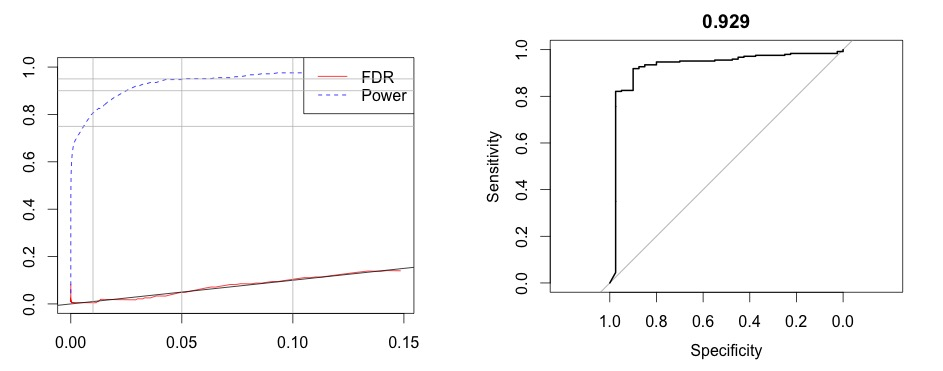
\includegraphics[width=\maxwidth]{figures/multivaraiteROC} \caption[]{ROC and FDR plots produced by the multivariate algorithm.}
\label{IL4}
\end{figure}

\subsection{Analysis Results}
Below are the covariance structure inferred from the data. The algorithm estimates the percentage of vaccines very accurately at $0.85$ (the correct one is $0.86$. I ran the analysis without the IL4+ cell subsets because it throws the analysis off a little bit- the FDR levels are still good but the power isn't as good. 

% latex table generated in R 3.1.0 by xtable 1.8-2 package
% Fri Nov 11 13:05:21 2016
\begin{table}[ht]
\centering
\begin{tabular}{rrrrrrr}
  \hline
 & 1 & 2 & 3 & 4 & 5 & 6 \\ 
  \hline
4+/CD154+ & 2.29 & 1.99 & 0.66 & 1.76 & 0.54 & 1.56 \\ 
  4+/IFNg+ & 1.99 & 1.96 & 0.49 & 1.61 & 0.42 & 1.51 \\ 
  4+/IL2+ & 0.66 & 0.49 & 0.66 & 0.40 & 0.31 & 0.50 \\ 
  4+/IL17a+ & 1.76 & 1.61 & 0.40 & 1.54 & 0.27 & 1.37 \\ 
  4+/MIP1B+ & 0.54 & 0.42 & 0.31 & 0.27 & 0.81 & 0.35 \\ 
  4+/TNFa+ & 1.56 & 1.51 & 0.50 & 1.37 & 0.35 & 1.45 \\ 
   \hline
\end{tabular}
\caption{Covariance Between Random Effects in the RV144 Dataset - Multivariate Analysis.}
\label{multiCovTable}
\end{table}

% latex table generated in R 3.1.0 by xtable 1.8-2 package
% Fri Nov 11 13:07:32 2016
\begin{table}[ht]
\centering
\begin{tabular}{rrrrrrr}
  \hline
 & 1 & 2 & 3 & 4 & 5 & 6 \\ 
  \hline
4+/CD154+ & 1.00 & 0.94 & 0.53 & 0.94 & 0.39 & 0.86 \\ 
  4+/IFNg+ & 0.94 & 1.00 & 0.43 & 0.93 & 0.33 & 0.90 \\ 
  4+/IL2+ & 0.53 & 0.43 & 1.00 & 0.39 & 0.42 & 0.51 \\ 
  4+/IL17a+ & 0.94 & 0.93 & 0.39 & 1.00 & 0.24 & 0.92 \\ 
  4+/MIP1B+ & 0.39 & 0.33 & 0.42 & 0.24 & 1.00 & 0.32 \\ 
  4+/TNFa+ & 0.86 & 0.90 & 0.51 & 0.92 & 0.32 & 1.00 \\ 
   \hline
\end{tabular}
\caption{Correlations Between Random Effects in the RV144 Dataset - Multivariate Analysis.}
\label{multiCorTable}
\end{table}



\begin{figure}
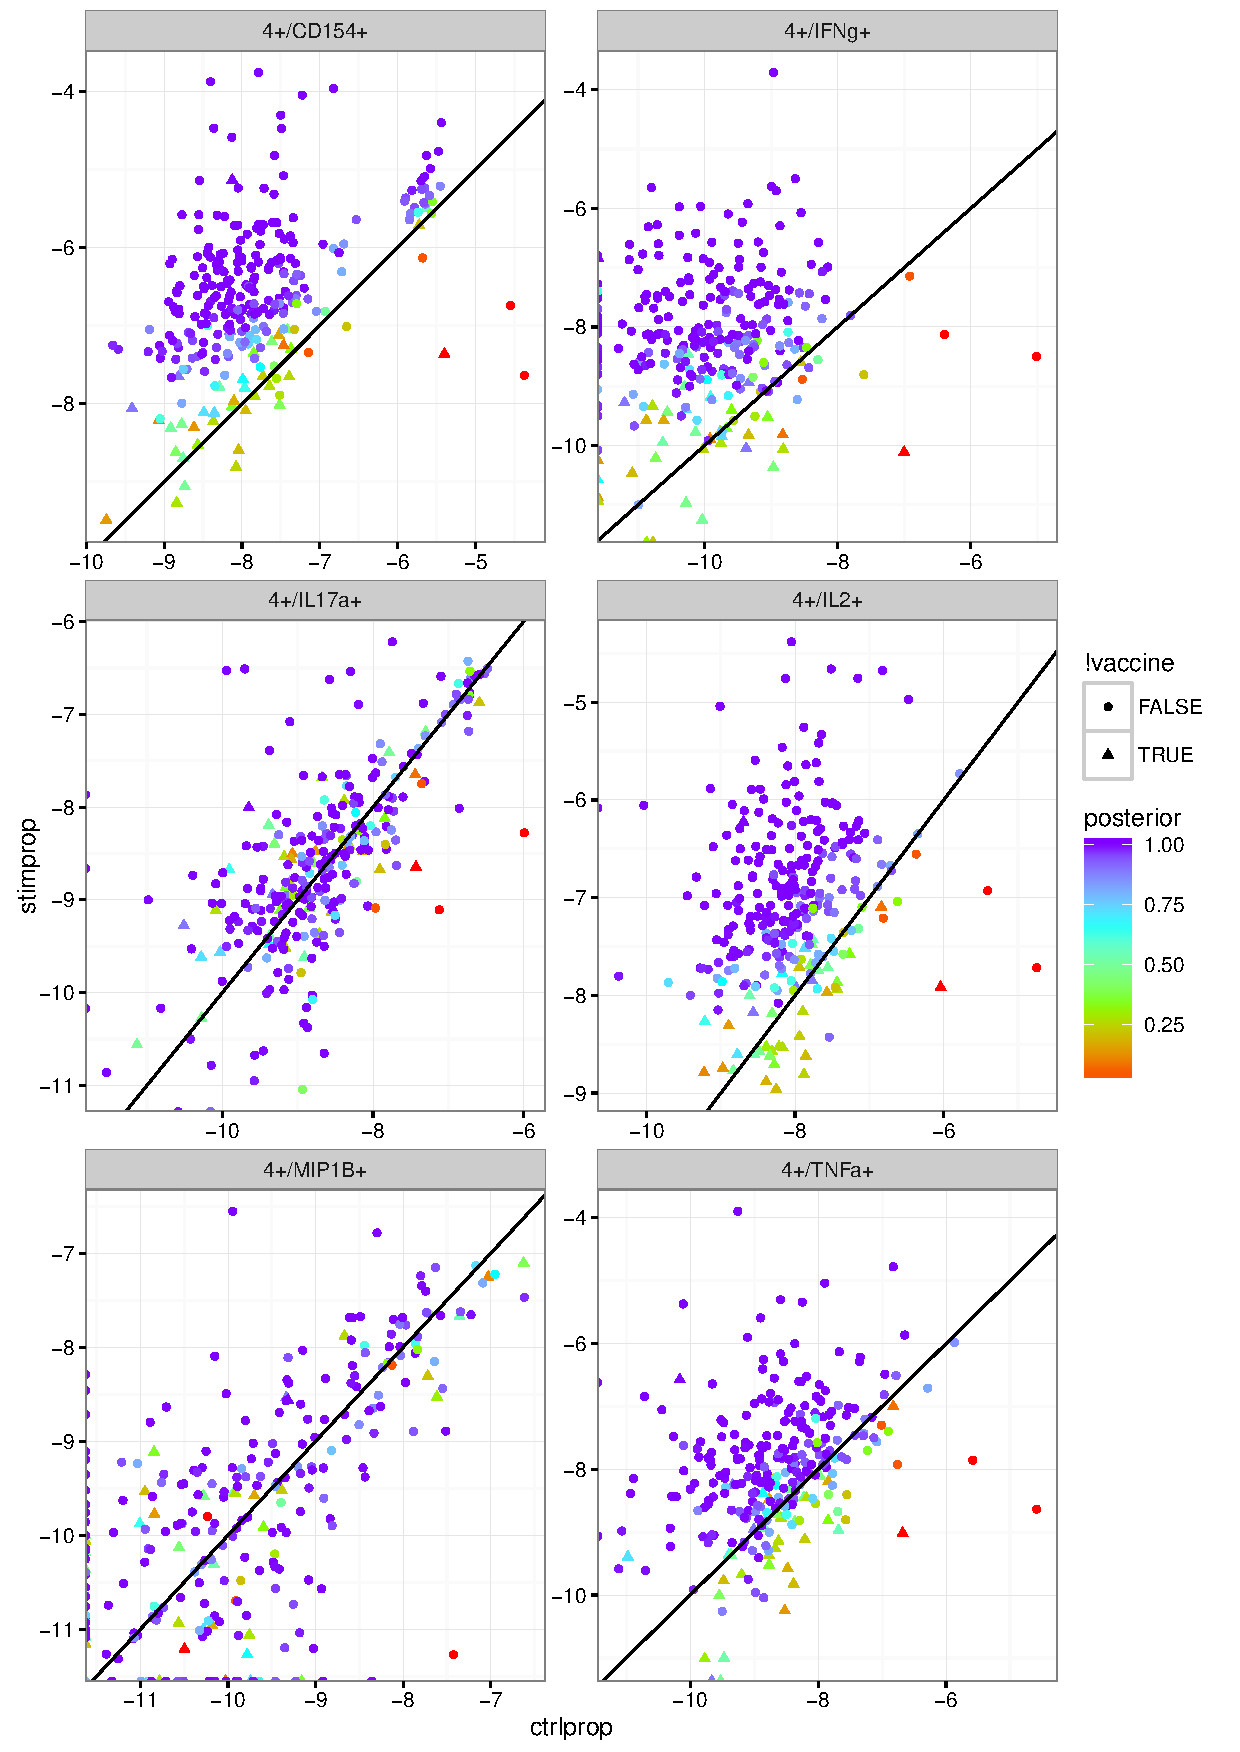
\includegraphics[width=\maxwidth]{figures/multivariatescatter} \caption[]{Scatter plots with posterior probabilities as produced by the multivariate algorithm.}
\label{IL4}
\end{figure}







\section{Modeling Subset Response}
The framework developed so far allows for the modeling of differential response at the subject level- an approach suitable for classifying subjects as responders/non-responders. It may also be of interest to model response at the cell-subset level. Such analysis may be more appropriate for understanding which cell subsets participate in the immune response. 

It is quite clear that the nested EM algorithm developed previously will not be suitable for such analysis. To see why, consider the joint modeling of a non-trivial number $k$ of cell-subsets, where for each cell subset a subject can be a responder or a non-responder. Denote by $z_{ik}$ a random variable taking the value of $1$ if the $i$th subject is a responder for the $k$th cell-subset or $0$ otherwise. We must assign each subject to a 'response cluster', where such an assignment can be represented as a binary vector of length $K$. The posterior probability of a realization of such a cluster is given by:
\begin{equation}\label{expsum}
P(z_{i} | y_{i}) = \frac{ f(y_i | z_{i}) P(a) }{ \sum_{ b \in \{0,1\}^{K}} f(y_i | b) P(b)},
\end{equation}
where $f(y_i | z_{ik})$ a is an integrated mixture density. The sum in the denominator of \eqref{expsum} is a sum over $2^{K}$ elements which may become computationally expensive even for datasets of modest size. An additional reason for why the nested-EM algorithm is an unattractive solution for estimating this model is the fact that previously, we estimated a random effect for every possible cluster assignment for each subject (there were two such assignments). In the presence of $2^K$ possible assignment this is no longer an attractive option. 

Recall that for the nested-EM algorithm we sampled a cluster assignment for each subject at each iteration. This, as an alternative to estimating a regression weighted by posterior probabilities. Here, we can use posterior sampling in order to avoid computing the sum at the denominator of equation \eqref{expsum}. Under the assumption that we are able to compute the mixture density efficiently, consider the following Gibbs sampling scheme.  At the $t$th iteration, for the $k$th cell-subset, sample an assignment with probability:
\begin{equation}\label{postGibbs}
P(z_{ik} = 1 | y_i, z_{i,-k}) = 
\frac{f(y_i | z_{ik} = 1, z_{-k}) P( z_{ik} = 1, z_{-k})}
{\sum_{l=0}^{1} f(y_i | z_{ik} = l, z_{-k}) P( z_{ik} = l, z_{-k})}.
\end{equation}

The sampling scheme described in \eqref{postGibbs} is simple and could be expected to explore the space of possible assignments in a reasonably efficient manner. However, given that the number of the subjects in a vaccine study is typically smaller, it is unlikely that we will have enough information to estimate $P(z_{i})$ in a reasonable manner without assuming a model for the joint distribution of the subset-specific response. 

A common model for the joint distribution of a binary random variable is the Ising model, which assumes that:
$$
\log P(z_i) = \sum_{k=1}^{K} z_{k} \eta_k + \sum_{k=1}^{K - 1}\sum_{l=k + 1}^{K} z_{k} z_{l} \gamma_{kl} + C,
$$
where $C$ is a normalizing constant. In general, the Ising model has $K + K(K-1)/2$ parameters to estimate, rather than the $2^{K}$ parameters we would have estimate otherwise. However, this number is still likely to be too large for the typical dataset of interest. As a simplified model, we can consider the following model:
 $$
\log P(z_i) = \sum_{k=1}^{K} z_{k} \eta_k + \sum_{k=1}^{K - 1}\sum_{l=k + 1}^{K} z_{k} z_{l} \gamma + C.
$$
Here, $\eta$ is a parameter vector which describes the probability of a response in each cell subset and $\gamma$ describes the dependence between the cell-subsets. To better understand the exact role $\gamma$ plays, write:
$$
\log P(z_{ik} = 1| z_{-k}) = z_k\eta_k + \sum_{l\neq k} z_{l} \gamma + \tilde{C}.
$$
That is, if $\gamma > 0$ then a response is more likely at the $k$th if a response is observed in other cell-subsets, and if $\gamma < 0$ then the converse holds. This could be a helpful model for our purposes as it is likely that a subject is a non-responder in all cell-subsets or a responder in several. Another more flexible option is to estimate a sparse graphical model via regularization.

Given this model, the question remains of how to perform estimation. Here again we use a Monte-Carlo EM. In the Stochastic E-Step, for a subject $i$, we will sample from the joint posterior distribution of the random effect vector $\nu$ and the assignment vector $z$. For $l \in \{1,...,L\}$: 
\begin{itemize}
\item Sample random effect:
	\begin{itemize}
	\item Sample proposal:
	$$
	v_l^{t} \sim f(\nu_l | \nu_{1}^{t},..,\nu_{l-1}^{t}, \nu_{l+1}^{t-1},...,\nu_{L}^{t-1})
	$$
	\item  Accept with probability:
	$$
	\frac{f(y | \nu^{t}, z^{t})}{f(y | \nu^{t-1}, z^{t-1})} 
	\frac{f(\nu_l^{t-1}|\nu_{-l}^{t})}{f(\nu_l^{t-1}|\nu_{-l}^{t})}
	$$
	\end{itemize}
	
\item Sample assignment from:
$$
z_l^{t} \sim P(z_l = 1 | y, z_{-l}^{t}, \nu^t)
$$
\end{itemize}
For each subject we keep $M$ samples. At the M-Step we maximize the likelihood:
$$
\sum_{i=1}^{n}\sum_{m=1}^{M} \log f(y_i | \nu_i^m, z^m_i)  +
\sum_{i=1}^{n} \sum_{m=1}^{M} \log f(\nu_i^m)
$$$$
+ \sum_{i=1}^{n}\sum_{m=1}^{M}\sum_{l=1}^{L} \eta_l z_{il}^m
+ \sum_{i=1}^{n}\sum_{m=1}^{M}\sum_{l=1}^{L-1}\sum_{k=l+1}^{L} \eta_l z_{il}^m z_{ik}^{m} + C.
$$












\end{document}
